\documentclass[a4paper, 12pt, oneside]{report}
\usepackage {tcdthesis}
\usepackage {verbatim}
\usepackage {acronym}
\usepackage {tabu}
\usepackage {url}
\usepackage {minted}
\usepackage {graphicx}
\usepackage [colorlinks]{hyperref}
\usepackage {fancyhdr}
\setlength{\headheight}{15pt}
\fancyhf{}
\rhead{\thepage}
\lhead{\textit{\nouppercase{\leftmark}}}
\hypersetup{
  colorlinks=true,
  linkcolor=black,
  urlcolor=black,
  citecolor=black,
}

\mastersthesis

\leftchapter
\doublespace

\renewcommand{\thesistitle}{Self-Sovereign Identity using Smart Contracts\\on the Ethereum Blockchain}
\renewcommand{\thesisauthor}{Zachary Diebold}
\renewcommand{\thesismonth}{May}
\renewcommand{\thesisyear}{2017}
\renewcommand{\thesistype}{Dissertation}
\renewcommand{\thesisdegree}{Master in Computer Science}
\renewcommand{\thesisauthorpreviousdegrees}{}
\renewcommand{\thesissupervisor}{Dr. Donal O'Mahony}
\renewcommand{\thesisacknowledgmenthead}{Acknowledgements}

\begin{document}
\thesistitlepage
\thesisdeclarationpage

\begin{thesisabstract}
Centralised identity services that exist today fail to operate transparently and protect the rights of users. Single points of trust present constant operational risks for both companies and individuals. Self-sovereign identity is a solution to address this, which specifies a user-focused approach that gives full control of an identity back to the individual. This paper proposes the blockchain, a secure and decentralised trust-less system, as the platform to achieve this. A proof-of-concept identity system for the \textit{Ethereum blockchain} is designed and developed in this paper. \textit{Smart contracts} are used to facilitate the secure storage and open processing of user data. It also presents a novel approach to the secure recovery of encrypted private data. Emphasis is placed on the implementation security, information privacy and data recovery procedures of the system. 
\end{thesisabstract}

\begin{thesissummary}
Digital identity systems that exist today are fragmented between service providers. Users need to duplicate their identity information between services, which reduces overall usability and increases the risk of data compromise. 

In addition, logically centralised providers that offer single sign-on methods restrict the end-user from controlling how their data is stored and processed. Trusting centralised entities to manage sensitive information can lead to issues like identity theft, data leaks and privacy breaches. 

Self-sovereign identity is a user-focused approach to identity management, that ensures full data control and transparency is retained by the individual. Self-sovereign identity also serves to protect the rights of  the users from the ever-increasing control of centralised entities.

Blockchain technology offers a decentralised, transparent and immutable platform on which to safely transmit and track assets like digital currency. The Ethereum blockchain extends this concept by allowing programmable pieces of code known as \textit{smart contracts} to be executed. These smart contracts can manage digital currency, and store and verify arbitrary data.

This paper investigates existing identity solutions, blockchain technology and decentralised systems. It then proposes a solution implemented with Ethereum smart contracts that encompasses the elements of cryptographic security, operational transparency, data autonomy and account recoverability. It is finally evaluated under a set of design objectives and comprehensive security considerations.

\end{thesissummary}

\begin{thesisacknowledgments}
I'd like to express my sincere gratitude to the following people for their support:

\begin{itemize}
	\item My supervisor, Dr. Donal O'Mahony, for his unwavering enthusiasm, immense guidance and continuous support throughout my research.
    \item The kind folks over at IPFS, uPort and the Solidity support channels for their extensive answers and technical advice.
    \item My fellow classmates in Integrated Computer Science, for their shared advice, dedication and energy during our college career.
    \item Finally, my loving family, for their constant encouragement, help and guidance throughout all my endeavours in life.
\end{itemize}
   
\end{thesisacknowledgments}

\tableofcontents
\listoffigures
\listoftables

\chapter*{List of Acronyms}
\addcontentsline {toc}{chapter}{List of Acronyms}
\begin{acronym}
  \acro{PKI}{Public Key Infrastructure}
  \acro{GDPR}{General Data Protection Regulation}
  \acro{KYC}{Know Your Customer}
  \acro{AML}{Anti-Money Laundering}
  \acro{IPFS}{InterPlanetary File System}
  \acro{OP}{OpenID Provider}
  \acro{RP}{Relying Party}
  \acro{SAML}{Security Assertion Markup Language}
  \acro{SSO}{Single Sign-On}
  \acro{MSD}{Mean Shortest Distance}
  \acro{CA}{Certificate Authority}
  \acro{UUID}{Universally Unique Identifier}
  \acro{JSON}{JavaScript Object Notation}
  \acro{OCSP}{Online Certificate Status Protocol}
  \acro{DLT}{Distributed Ledger Technology}
  \acro{MRZ}{Machine Readable Zone}
  \acro{DHT}{Distributed Hash Table}
  \acro{IPNS}{InterPlanetary Naming System}
  \acro{RPC}{Remote Procedure Call}
  \acro{BIP}{Bitcoin Improvement Proposal}
  \acro{PII}{Personally Identifiable Information}
\end{acronym}

\chapter{Introduction}
This section introduces the motivation for the dissertation work. The background to the field is explored, as well as the desired research objectives and possible challenges. Finally, the technical approach to implementing the planned work is outlined.

\section{Motivation}
\label{sec:motivation}
The concept of identity is fundamental to human activities. The identity of an individual, their attributes, and representation of \textit{the self} is understood worldwide regardless of culture. Psychological and social well-being is also said to be dependent on maintaining a stable personal identity \cite{sharma_self_2010}. 

Modern society binds the notion of individual identity with a legal identity, such as social security numbers, passports and driving licences. This binding leads to situations where one can lose their identity if the state rescinds it. It is especially apparent in the case of refugee crises, where migrants have difficulty living in countries in which they are not registered.

Digital identity represents entities such as people and organisations in an online context. In its current state digital identity is siloed between providers, necessitating the creation of many identities across the internet.

Due to this fragmentation, users eventually link multiple identities to their legal identity over time, which can pose risks of identity theft, privacy breaches and data leaks \cite{camp_economics_2012}.

As the digital world becomes more prevalent in everyday life and the quantity of internet-connected devices increases, the risks of trusting disparate centralised services become very high. As a result of this, an opportunity arises to redefine modern concepts of digital identity in a decentralised context.

\section{Research Objectives}
Self-sovereign identity is the notion that an individual should have complete authority over their digital identity and its data. It removes control from centralised entities and pushes it out to the edges of the network, the users themselves.

The core mission of blockchain technology is to provide a decentralised trust network. This can be mapped nicely onto the problems with centralised system trust in the identity landscape.

Thus, this dissertation proposes a system using the Ethereum blockchain, a decentralised application platform, to create a self-sovereign identity solution. Such a solution, in pursuit of this goal, should conform to the following requirements:

\begin{enumerate}
  \item \textbf{Data Security}: Identities and their corresponding attributes should be stored in a secure manner, to prevent data compromise. Access and modification of user data should be restricted to the sole owner of the data.
  \item \textbf{Interface Usability}: To interface with the system, it should not require prior knowledge of the underlying blockchain technology, key management procedures or encryption protocols. \ac{PKI} is an example of a system that has not reached widespread consumer adoption, partly due to poor system usability \cite{straub_usability_2006}.
  \item \textbf{Identity Verifiability}: Individuals should be uniquely identifiable in the system, and have the ability to prove ownership of their information. External entities should be able to attest to the attributes of an individual.
  \item \textbf{Account Recovery}: The system should allow for identity recovery in the case of device loss or data compromise. Revoked identities and attributes should also be discoverable by third parties.
  \item \textbf{Self-Sovereignty}: The storage of data should not depend solely on a centralised entity, and as such the identity should be under full control of the user.
\end{enumerate}

\section{Use Cases}
Such a self-sovereign system provides full autonomy over a user's personal identity, reputation and online presence. Example use cases for a decentralised self-sovereign identity platform are given below for context.

\begin{itemize}
  \item Users can maintain a single identity for connecting to online services, such as social networks or enterprise systems. The system provides authentication of the user to the online service to prove ownership of their identity. This allows controlled single sign-on without the need for transferring passwords or secret information, as only the proof is transmitted.
  \item Governments can attest to the citizenship status or legal attributes of citizens, to then verify them in later interactions. Self-sovereignty and portability of the data allows it to be used internationally across borders.
  \item Financial institutions can establish an improved \ac{KYC} process, to verify the legal identities of customers using their services. Liability is reduced by not storing raw customer data, while still complying with \ac{AML} regulation.
\end{itemize}

\section{Technical Approach}
The Ethereum blockchain, while operating in a similar manner to Bitcoin by facilitating currency transfers, can also store programs known as \textit{smart contracts}. These programs are compiled to machine code and immutably deployed to the blockchain, and are verified and appended to the shared public ledger of transactions. The application state stored in these smart contracts is transparent and verifiable, and the execution of contract code is supported by the decentralised network. 

Users in this system generate public and private keys corresponding to Ethereum wallets, and subsequently deploy Ethereum contracts containing their unique identifier. The generation and deployment of the smart contracts is done in the client, using a JavaScript framework for interfacing with Ethereum known as \textit{Web3.js}.

Identity attributes are be stored on the decentralised storage platform known as \ac{IPFS}, which allows for the data to be stored in a redundant and immutable manner.

As the core of the platform is the Ethereum smart contract, the client-side interface is seen as complementary and not central to the operation of the system. All the security and access-control features of the system are contained solely in the immutable contract code.
\chapter{Digital Identity}
\section{Introduction}
\subsection{Definitions}
Identity is a set of characteristics and attributes that describe an entity, that can then be used to uniquely identify it. Digital identity is the representation of an entity in a specific environment or context. It consists of unique identifiers, descriptive attributes and data claims related to the system for which it is issued.

To understand the variety of identity platforms that have existed over the years, some core concepts about identity should first be strictly defined.

\subsubsection{Identifiers}
An \textit{identifier} is a piece of information used to distinguish a distinct person or entity in the context of a system. As noted by security researcher Steve Riley \cite{riley_its_2006}, this is the user's answer to the question \textit{"Who are you?"}. An entity can possess multiple identifiers associated with different functions. An example of an identifier for a person, is their name, social security number, email address or credit card number.

\subsubsection{Authentication}
\textit{Authentication} of an entity is performed by proving an association between a user and their identity. Again, this answers the question \textit{"Ok, how can you prove it?"}. The system will present a challenge that the user must answer with secret or private information known as the \textit{authenticator}. Authenticators can include passwords, PINs and private keys. In the case of passwords, the system compares against secret information it already holds. For private keys, this is different, as it only needs to verify a proof that you know the secret value and does not require its transmission.

Multi-factor authentication is commonly used to enhance system security and has been noted by recent research \cite{schneider_system_nodate} to consist of the following three methods:
\begin{enumerate}
	\item \textbf{Something you know}: This is the most common form of an authenticator, like a password.
	\item \textbf{Something you have}: This is a physical object, like a smart card or hardware key.
	\item \textbf{Something you are}: This is an intrinsic attribute of the entity, such as a fingerprint or biometric value.
\end{enumerate}

\subsubsection{Authorisation}
\textit{Authorisation} is done to request permission to perform an action based on a particular identifier or attribute. This can be seen as the user asking the question \textit{"What can I do?"}. A system performs authorisation of the user against a database or rule set before approving their requested actions. The authenticated identity of the user is stored by the system, once authorised, to enable future access to resources. This often consists of issuing a time-bound token or ticket to the user.

\subsubsection{Attributes}
\textit{Attributes} are pieces of data related to an entity that helps describe it. The values of which can be persistent or temporary. An example of the attributes of a person are date of birth, gender, employer and physical address.

\subsubsection{Attribute Attestations}
\textit{Attestations} or \textit{claims} are verifications that establish the mapping from a given user attribute to their identity. In many identity systems, identity authentication precedes the attribute verification process, in order to confirm that the correct identity is being presented. An example of an attribute attestation is a bank attesting to the credit score of a customer, or the police attesting to the name and date of birth of a citizen.

\subsection{Know Your Customer}
\acf{KYC} is the process by which a business verifies the identities of its customers. This is often linked closely with \acf{AML} state regulation and is enforced with the view to reducing criminal activity and fraud. Accurate identification of customers is required by law and mistakes are met with hefty penalties \cite{nasiripour_uk_2012, financial_conduct_authority_fca_2017}.

Therefore, businesses in the financial sector have a strong economic incentive to ensure that stakeholders are accurately identified in their systems. This incentive speeds up the pace of innovation in this sector, in search of improved procedures and enhanced technology.

\subsection{Self-Sovereign Identity}
Self-sovereign identity is a user-focused approach to identity, favouring the rights of the end-user. It proposes that individuals should have full control and autonomy over their identity and its data. These are succinctly defined by the cryptographer Christopher Allen \cite{allen_path_2016} with his ten pillars of self-sovereign identity:

\begin{enumerate}
	\item \textbf{Existence}: Users must have an independent presence in the system, and it must be an extension of their existing personal identity.
	\item \textbf{Control}: Users are the ultimate authority over their identity, how it is used and how data is disclosed.
	\item \textbf{Access}: Users must have easy access to their own data, without it being hidden or kept from them.
	\item \textbf{Transparency}: Systems that manage the data, and the algorithms that analyse it, must be transparent, open-source and public.
	\item \textbf{Persistence}: Identities must have the ability to be long-lived or permanent, at the discretion of the user.
	\item \textbf{Portability}: Identities cannot be held by a single entity, trusted or not, and must be transportable between services.
	\item \textbf{Interoperability}: Identities must have the ability to operate across systems, companies and borders.
	\item \textbf{Consent}: Sharing of user data must be done with explicit consent and knowledge of the user.
	\item \textbf{Minimalisation}: Data that is disclosed or shared should be minimised where possible. This is helped by the introduction of selective disclosure and zero-knowledge techniques.
	\item \textbf{Protection}: The rights of the user must be central to the system, and be independent, decentralised and censorship-resistant.
\end{enumerate}

These pillars may seem to be strict, but all ten are required if a truly self-sovereign system is to be produced. The \ac{GDPR} in Europe \cite{european_parliament_eu_nodate} that will take effect in 2018 will legislate for some of these principles and puts the importance of this research into context.

Other research organisations like ID2020 \cite{identity2020_systems_inc_id2020_nodate} are already attempting to tackle these issues on a global identity scale, and are doing so by developing new technology, lobbying governments, and advocating for the principles outlined above.

\section{Identity Management Systems}
\subsection{Overview}
Identity management systems were introduced to address some of the risks outlined with siloed providers in Section \ref{sec:motivation}. They attempt to solve the fragmented multi-account problem by centralising the user's identity data and standardising its usage. Some recent approaches are summarised below.

\subsection{OpenID}
OpenID is a protocol that was developed in 2005 by Brad Fitzpatrick, the creator of the popular blogging platform LiveJournal \cite{fitzpatrick_distributed_2005}.
It allows users to create an account with an identity provider that supports the standard, known as the \ac{OP}. The user can then use this account to authenticate with a third party service or \ac{RP}, without managing multiple usernames and passwords.

The user must be sure to select a site that is reputable and long-lived, to ensure that the identity safely persists over time. OpenID removes the requirement for remembering passwords across many sites, but still leaves the users trusting their OpenID identity provider with important data. Accounts could be modified or deleted at any time at the discretion of the identity provider, so it does not provide much sovereignty to the user.

This inherent centralisation, coupled with the fact that users are forced to rely on an abstract identity system, eventually caused OpenID to lose prominence on the web \cite{gilbertson_openid:_2011}.

\subsection{SAML}
\ac{SAML} \cite{oasis_security_services_saml_2005} is an XML-based open standard for web browser \ac{SSO} using secure tokens. It is commonly used in enterprise contexts for authentication between applications and a company Active Directory. Identity providers pass identity information to service providers through digitally signed XML documents.

The four main components of the standard are as follows:
\begin{enumerate}
	\item Assertions - These consist of authentication assertions used to prove the ownership of an identity, and attribute assertions used to generate specific information about the person.
    \item Protocols - These define how certain \ac{SAML} elements like assertions are packaged for transfer and also the processing rules associated with them.
    \item Bindings - These define the raw transport methods used to transmit the authentication data. These can include HTTP GET, HTTP POST and SOAP.
    \item Profiles - These define in detail how assertions, protocols and bindings combine to form a use case. \ac{SAML} 2.0 introduces many more profile contexts, including allowing the request to begin from the service provider itself.
\end{enumerate}

The verbosity of the \ac{SAML} standard and the fact that it can require extra infrastructure to support the transfer protocols \cite{dennis_updated_2015} has restricted its deployment to legacy enterprise environments. 

\subsection{OAuth}
OAuth \cite{hammer-lahav_oauth_2010} was introduced to allow a user to grant access to private resources connected to their identity. This is done without sharing private identity details or passwords between services. A long-lasting access token is specified by the protocol, which can be used by entities for continued access to user resources. 

An example of this would be a user granting access of their Twitter or Facebook account to an external service, perhaps to allow it to make posts or gather analytics. The authorisation procedure and access token used by this external service would be managed using the OAuth specification.

OAuth is distinct from OpenID, as although it shares the common architecture of redirection for obtaining authorisation, it only manages the access control of resources. OAuth does not have a concept of identity and does not provide identity authentication.

OAuth and its updated standard OAuth 2.0 are both still in active use by many social networks and dependent applications, but it does not provide much value to the end-user in terms of identity sovereignty or control.

\subsection{Discussion}
Identity management systems, while attempting to reduce risks in the field, can still suffer from failure \cite{mimoso_office_2016, low_serious_2014}.This is owed to their inherent centralisation of data and resources. Therefore, there exists a gap in the state of the art for a management system not owned and managed by a single entity.

\section{Public Key Infrastructure}
\subsection{History}
\ac{PKI} is a system for managing public-key encryption and digital certificates. It helps facilitate the secure transfer of information, and it authenticates parties operating over an insecure network. The principles behind this technology known as \textit{asymmetric cryptography} were developed in 1976 by Whitfield Diffie and Martin Hellman \cite{diffie_new_1976}. This was also explored in 1978 by another set of mathematicians when the RSA algorithm for asymmetric key generation was published \cite{rivest_method_1978}.

In asymmetric cryptography, a public and private key are first generated. The relationship between these is such that data encrypted with one can only be decrypted by its matched pair. The public key can be widely distributed for identification of an entity, while the private key acts as a verifiable authorisation mechanism of that identifier.

\subsection{Certificates}
Critical to the functioning of \ac{PKI} is the use of digital certificates, which give key pairs meaning and establish the identity of entities within a given context. Certificates contain information about the issuing party, the subject of the certificate, the expiry of the content and a digital signature. This digital signature is added to prove that the issuing party verified and signed the certificate with their private key. 

The authenticity and integrity of such certificates and how they are issued must be protected, to maintain a level of trust in the system. Centralised parties that issue certificates can be susceptible to errors or failure, such as DigiNotar \cite{the_associated_press_hacking_2011} and Symantec  \cite{ayer_misissued/suspicious_2017}, so revocation procedures in the given system should be robust.

\subsection{Certificate Authorities}
A \ac{CA} manages the lifecycle of digital certificates and acts as an entity that both the subject of the certificate and the party relying on it trusts. Root authorities are \acp{CA} that are inherently trusted by the end user and are pre-installed on devices and browsers. \acp{CA} are fundamentally centralised entities that perform individual validation for every entity that wishes to be certified.

Certificates that are presented by a party can be traced back to a root authority to verify authenticity. This chain of trust underpins the \ac{PKI}, and all transactions and exchanges of information are protected by the certificates it contains.

\subsection{Attribute Authorities}
Attribute Authorities \cite{farrell_internet_2002} are similar to Certificate Authorities, but they exist when the separation between public keys and attributes is necessary. They can issue attribute certificates, which are used to control access to systems or resources. 

This distinction from public key certificates is useful when the lifetime of an attribute certificate is different to that of the parent certificate. It is also sometimes required when the \ac{CA} cannot authorise a user for accessing a particular resource, so a secondary authority must do so instead. The authorisation information for an entity is thus logically separated from its identity for these reasons.

\subsection{Signatures}
Digital signatures act as a proof for authenticity and integrity of a piece of data. It certifies that digitally signed information was produced by a trusted source and has not changed since the signature. Data is passed through a hashing algorithm which produces a fixed-length output that cannot be easily reverse engineered. This hash is then encrypted with the private key of the entity and sent with the data. The receiver can validate the integrity of the message by passing the data through the same hashing function and matching it with the decrypted signature.

\subsection{Web of Trust}
\label{sec:web-of-trust}
The Web of Trust \cite{the_free_software_foundation_gnu_1999} concept was introduced with PGP version 2.0, and it is a decentralised model of identity reputation achieved via a network of trusted parties. Users build up a reputation by having their keys verified and signed by their peers. A chain of trust can then be followed back to a locally trusted user when presented with a new key.

A physical meeting in person is usually done to verify the mapping from an individual to their private key before creating a signature. Key signing parties \cite{brennan_keysigning_2008} exist for this purpose, where multiple individuals sign each other's keys after identity verification.

The \ac{MSD} value is used to calculate how trusted a given key is, by finding the average shortest distance or number of hops from the user's trusted keys.

\subsection{Discussion}
The core concepts of \ac{PKI} are widely used on the internet to secure transactions and files. Data transfer over the HTTP protocol is encrypted and executable application files are signed using certificates. 

\ac{PKI} is suitable in the context of delivering content from enterprise to end-users, but it does not work well the other way around. Key distribution, management and revocation issues have prevented \ac{PKI} from being widely deployed as a user-focused identity system.
\chapter{Blockchain}
\section{Introduction}
\subsection{History}
The technology behind the blockchain was first conceived with the release of Bitcoin in 2008 by Satoshi Nakamoto \cite{nakamoto_bitcoin:_2008}. The Bitcoin blockchain is a revolutionary idea that allows peer-to-peer transacting of digital currency in a trust-less environment. It uses cryptographic signatures to verify exchanges of currency, and a distributed ledger to maintain the order of transactions.

\subsection{Digital Wallets}
Digital wallets are used in the Bitcoin network to hold digital currency. All parties who hold a wallet have a public and private key pair. This is similar to \ac{PKI}, which uses key pairs as an identification and authorisation mechanism. The public key is the address used to publicly identify the wallet and receive funds, while the private key is used to make transactions using the wallet and prove ownership. 

In a sense, the public key is an anonymous representation of identity on the network as it is not tied directly to an individual. However, research has shown \cite{ron_quantitative_2013, reid_analysis_2013} that a method known as \textit{chain analysis} can trace transactions as they propagate through the blockchain, thus implying that the network is instead pseudonymous.

\subsection{Transactions}
\begin{figure}[ht]
\centering
     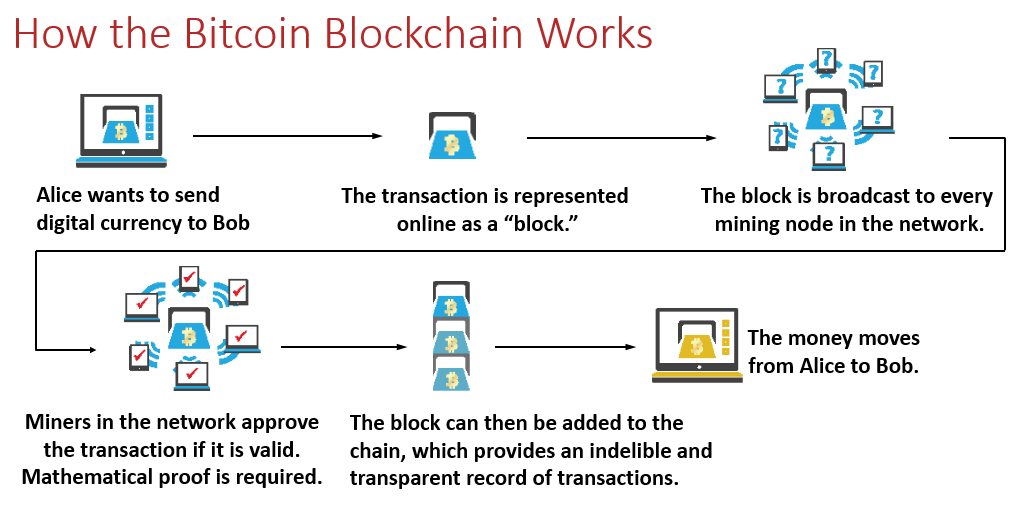
\includegraphics[width=1.0\textwidth]{./images/BitcoinTransaction.png}
      \caption[How the Bitcoin blockchain propagates transactions]{How the Bitcoin blockchain propagates transactions \protect\footnotemark}
       \label{fig:bitcoin-transaction}
\end{figure}
\footnotetext{Image source: D.Sleeter, "The Promise of Blockchain Technology," Jan. 2017. [Online]}

An example transaction is shown in Figure \ref{fig:bitcoin-transaction} above. If a user \textit{Alice} wishes to send another user \textit{Bob} digital currency from her wallet, she needs to first obtain the public address of Bob's wallet to create a new transaction. This transaction contains Bob's address, the payment amount, and the network fee. Alice must then sign this transaction with her private key, which proves to the network that she has cryptographic ownership of her corresponding wallet address. Alice then broadcasts this transaction on the blockchain, where it is received by other machines known as \textit{miners}.

\subsection{Distributed Consensus}
Bitcoin replaces a centralised payment ledger with a distributed one, but the problem arises of ensuring these transactions are ordered in a synchronised way. In the transaction between Alice and Bob above, the network needs to ensure that the coins being sent exist in Alice's wallet, and cannot be sent twice. This is referred to as the \textit{double spending} problem \cite{hoepman_distributed_2007}. 

A \textit{proof-of-work} verification system is used to tackle this. It specifies a certain algorithm which takes a non-trivial amount of processing power time to compute but conversely the solution is trivial to validate. 

When a transaction is broadcast to the network and received by a node, it is bundled with other unconfirmed transactions into a \textit{transaction block}. This block contains a list of transactions, a link to the previous block, and a random nonce number. This number is incremented until the computed hash of the block including this nonce begins with a specified number of zeros, thus providing a method of proof of work.

Calculating this hash correctly is computationally intensive, and ensures that a certain amount of computing power is required to validate a block. Once a block has been created with the desired hash, as shown in the figure above, it is broadcast to the network, and other nodes can verify its legitimacy by adding it to the end of their chain of blocks. This block is now considered \textit{valid}, and the order of transactions within the chain is thus preserved. 

In return for using computing power to verify blocks, the operator of the mining node receives some freshly generated Bitcoin currency in their wallet, as well as the network fees that users included in their transactions. This block reward began at \textit{50 BTC}, but it has been halved twice since to combat inflation and now stands at \textit{12.5 BTC} per block mined at the time of writing.

A key strength that comes with the ordering of transactions is that each transaction can be traced back to the original block where its source Bitcoin was minted. Before a Bitcoin node can start to mine and verify blocks of transactions, it must first download the entire history of transactions since the blockchain inception and verify each one independently. Only then does it begin to verify new transactions and add them to the blockchain.

\section{Ethereum}
Ethereum was released as an \textit{"alternative protocol for building decentralised applications"} \cite{buterin_ethereum:_2014}. It builds on the blockchain features described in Bitcoin above, by adding programmability and scalability to the network. Ethereum does not just represent a digital currency, as Bitcoin does, but also allows many other use cases to be stored as application-level code on the blockchain.

\subsection{Smart Contracts}
Ethereum contains smart contracts, which are computer programs compiled and stored in the Ethereum blockchain. These are assigned addresses and can receive currency transactions just like standard wallets, but their functions can also be initiated with special types of function call transactions.

Smart contracts can accept parameters, store state, manipulate internal state as a result of function calls, and return data in responses. This added functionality is not present in the Bitcoin blockchain, and it comes with distinct advantages. Application logic is performed and displayed transparently on the public blockchain, the internal state is available openly for scrutinising, and the operations are completely autonomous. They provide cryptographically auditable, append-only ledgers for building a new era of decentralised applications.

\subsection{Ethereum Virtual Machine}
Ethereum miner nodes are required to verify all state changes as blocks are propagated through the network. Application level code that is executed within smart contracts is considered a state change that is performed by the network via consensus. 

To achieve this consensus through code execution, the \textit{Ethereum Virtual Machine} was developed. This allows mining nodes to run code of arbitrary algorithmic complexity in a deterministic manner, and to reach consensus on the outcome of the computation. Smart contract operation is parallelised across all nodes in the network, which ensures fault tolerance, zero downtime, and permanent irrefutable state changes.

In the same way that Bitcoin miners accept network fees for verifying transactions, Ethereum miners that compute smart contracts receive fees for program execution. This is called the \textit{gas price} of the transaction. The sender must pay for each line of code the program executes, including computation, events and storage. This is to discourage attacks like infinite loops in code from affecting the network.

\subsection{Discussion}
Ethereum provides secure transfers of value, auditable and autonomous program execution, fault-tolerant redundant storage, and an immutable record of information. This makes it a powerful platform on which to tackle global problems in a new decentralised paradigm. It's been considered as the first \textit{Global Computer}, capable of operating completely censorship-free and across international borders.

The Ethereum platform has been chosen for the system design in this paper as it addresses many of the problems with centralised identity management. This is further outlined in the Solution Overview and Implementation details in Chapters \ref{chp:solution-design} and \ref{chp:implementation}.

\section{Decentralised Storage}
After the introduction of the blockchain, decentralised storage solutions have arisen that offer redundant hosting of long-form information and files. They present the following advantages:
\begin{itemize}
	\item Low-latency data retrieval
    \item Efficient content caching
    \item Reliable fault-tolerant storage
    \item Censorship resistance
    \item File versioning and archival functionality
\end{itemize}
Some notable implementations are discussed below.

\subsection{IPFS}
\ac{IPFS} \cite{benet_ipfs_2014} is a content-addressed distributed file system supported by a peer-to-peer network of machines. It can operate on any transport protocol and uses \acp{DHT} for peer identification and routeing. It provides cryptographic-hash content addressing, file integrity, and filesystem encryption and signing.

\ac{IPFS} also supports a name service known as the \ac{IPNS} for the persistent naming of dynamic content. This allows for routeing of a static name to the hash of a file and is based on access control concepts from \ac{PKI}.

The function of \ac{IPFS} is similar to Bittorrent, whereby nodes serve local copies of content to the network. When files are requested, the local node caches the response and continues to seed the file back to the network. If all nodes serving a file go offline, then the file is no longer available. An economic incentive such as Filecoin \cite{filecoin.io_filecoin:_2014} has been suggested as an addition to the protocol, which would encourage nodes to continue serving content for financial reward.

\subsection{Swarm}
Swarm \cite{noauthor_swarm_nodate} is a distributed storage platform and content distribution network similar to \ac{IPFS}. Both projects provide decentralised storage of content-addressed files split into chunks.

Swarm is distinct in that it runs on the Ethereum peer-to-peer networking layer, and was developed in the context of close integration with the Ethereum blockchain. It also supports incentivised system benefits through smart contracts native to Ethereum via the pool of network peers.

Swarm is slightly behind \ac{IPFS} in terms of development and global reach, and it is possible that the two projects could integrate together sometime in the future \cite{ethersphere_ipfs_2017}.

\subsection{Discussion}
Decentralised storage is cheaper than using Ethereum contract storage, and it does not bloat the network with large amounts of data. It is therefore seen as valuable to use an external decentralised storage system for the solution proposed in this paper.

\section{Blockchain Identity Systems}
\label{sec:blockchain-identity}
\subsection{Blockstack}
Blockstack \cite{blockstack_inc._blockstack:_2017} is a decentralised identity, discovery and storage platform, built on blockchain technology. It makes use of virtualchains \cite{j_nelson_extending_2016} that allow the output of arbitrary state machines to be pinned to underlying blockchain infrastructure. 

Blockstack is similar to Ethereum in that it supports decentralised applications, but instead performs its computation off-chain. The underlying blockchain technology is used to authenticate an application before it is run by the user. Applications are not Turing-complete by design, but they can interface with the Turing-complete Ethereum blockchain by use of a virtualchain.

Blockstack supports an identity project known as Onename, which allows users to register an identity on the Blockstack network. This features peer-to-peer identity attestations and verifications. Originally Onename used the Namecoin blockchain as its infrastructure, but changed to Bitcoin instead in response to centralised-mining and spam issues with Namecoin \cite{kyle_torpey_3_2015}. 

Although Onename supports a decentralised blockchain-based identity service, it still relies on off-chain computation using Blockstack with many layers of resolvers and verifiers \cite{onename_introducing_2015}. The lack of a stable and transparent network supporting the system reduces the usefulness of the project.

\subsection{Estonian e-Residency}
The Republic of Estonia released a state digital identity system known as e-Residency in 2014 \cite{the_digital_society_estonian_2014}. It is a transnational secure identity offered by the government and supported by a physical smart card.

Citizens apply to the government with their legal information, including copies of their fingerprints, before being issued a digital identity. Residents can use the system for company registration, banking, payment services and document signing. 

The cards use 2048-bit RSA encryption for document signing and verification. Legal documents can be digitally signed using this technology, with the full support of the Estonian legal system. The system currently does not use blockchain-based infrastructure, but it has partnered with initiatives like Identit.ee \cite{noauthor_identit.ee_nodate} and Bitnation \cite{bitnation_estonia_2015} to pursue this in the future.

\subsection{Evernym}
Evernym \cite{smith_identity_2016} is an identity system built on the permissioned \ac{DLT} known as Sovrin, which is dedicated solely to decentralised identity.

The Sovrin network is supported by the Sovrin Foundation, and it consists of interconnected nodes forming a consensus on a shared ledger. Users create self-sovereign identities with personal attributes, and request claims from trusted third parties to build reputation.

Currently, there is no financial incentive to host a Sovrin node, so the majority of the network is research-focused. The network plans to introduce premium claims in the future to provide rewards to nodes that distribute and verify identities \cite{sovrin_foundation_sovrin_nodate}. 

\subsection{ShoCard}
ShoCard \cite{shocard_inc._shocard:_2016} is a digital identity application focusing on user identification in the travel sector. It offers a mobile application for storing identities, while also pinning hashed and signed identity data to the Bitcoin blockchain.

Users scan their document with the application, which reads each \ac{MRZ} and stores an encrypted version on the device. Each field is then one-way hashed, signed with the user's private key, and published to the blockchain.

Disclosure of user data is done by encrypting the local copy of information with the receiver's public key and transferring it via a QR code. The receiver can then validate the information against the signed version published on the blockchain. 

ShoCard specifies that the receiving party, such as an airline gate agent, checks the digital copy against the physical passport before proceeding. The airline can then create certification records confirming this physical and digital link, and hand them back to the user. This is referred to as a \textit{travel token}. The user can then present this token at subsequent passenger checks to streamline verification. However, each checkpoint is still required to compare the token against the blockchain. This is done to check for continued validity and possible revocation of the token.

ShoCard presents a useful data disclosure process, ensuring transferred data is checked against the blockchain during each transaction. It fails to support any key or identity recovery protocols, however, and is inherently tied to identity supported by physical documents only.

\subsection{uPort}
\label{sec:uport}
uPort is a self-sovereign identity platform built on the Ethereum blockchain. At its core, it utilises a network of smart contracts for each user and offers a mobile application and accompanying developer libraries.

The uPort mobile application generates a public and private key for a user and deploys smart contracts to represent their identity. It deploys what is known as the \textit{Proxy Contract} to represent the user's unique identifier, the \textit{Controller Contract} to provide identity access control logic, and the \textit{Recovery Quorum Contract} to facilitate the recovery of the user's identity. It also stores pointers to these contracts in a centralised \textit{Registry Contract}.

uPort presents a novel recovery concept for digital identity, where a quorum of the user's friends can collaborate to restore access to an identity. Friends can vote to replace the ownership key of an identity with a newly-generated one, and the identity contract logic performs this request when a majority consensus is reached.

uPort retains some centralised elements, as it uses a centralised messaging server to transfer attribute information from a user's device, a push notification system and application manager. It also requires the use of a central registry to log the mapping of user public keys to unique identifiers for convenience. These elements are deemed necessary by the project for initial user onboarding, but have the potential to be removed in the future \cite{braendgaard_response:_2017}.

In addition, uPort does not support the recovery of private data, as this is stored off-chain on the user's device. Sensitive data cannot be stored in public form on the blockchain without first being encrypted. This research identifies a possible approach to allow this data to be recovered.

\subsection{Discussion}
There are many approaches to providing self-sovereign in the digital space, with promising blockchain implementations. The primary areas of interest that remain unsolved are completely decentralised systems that support the recovery of private identity data. 

The focus of this research is to propose a solution that builds upon the advancements of existing work in the field, and to use stable and transparent blockchain architecture with complete privacy and adequate recoverability.
\chapter{Solution Design}
\label{chp:solution-design}
The proposed solution builds on some of the advancements in the field of self-sovereign digital identity as shown in Section \ref{sec:blockchain-identity}. It focuses on a decentralised model of data storage and communication, with privacy-preserving features and identity recovery.

\section{System Overview}

The system is comprised of three primary parts:
\begin{enumerate}
	\item \textbf{Smart Contracts}: These are immutable programs stored on the Ethereum blockchain. Their function is to store the unique user identifier, a pointer to the user's data and the logic for modifying this data.
    \item \textbf{Data Storage}: The user data is stored in \ac{JSON} format on the decentralised storage platform \ac{IPFS}, with a reference to this data given to the smart contract.
	\item \textbf{Device Key Pair}: This is a public and private key pair stored on the end user's device, used for authenticating the user and allowing them to access and update their identity.
\end{enumerate}

\subsection{Smart Contracts}
The smart contracts are the core of the user's identity. There are two smart contracts that the user deploys onto the blockchain, that represent their identity.

The source code for these contracts is necessarily simple, to facilitate robust code execution and transparent auditing. This can be viewed in detail in Appendices \ref{apd:identity-contract} and \ref{apd:recovery-contract}.

\subsubsection{Identity Contract}
This contract contains the authoritative version of the user's identity, as well as the access control logic for attribute modification. Once this contract is deployed to the blockchain, the reference address that is returned is the user's \ac{UUID}. This address never changes, and it ensures the user maintains a persistent identifier even if their personal access keys are recovered or updated.
The data stored in the contract is shown in Table \ref{tab:identity-contract} below.

\begin{table}[h]
	\centering
    \begin{tabular}{|p{3cm}|p{8cm}|}
        \hline \textbf{Contract Data} & \textbf{Purpose} \\
        \hline owner\_key & Public key of the identity owner \\
        \hline recovery\_contract & Address of the associated recovery contract \\
        \hline ipfs\_hash & Hash pointing to the user data in \ac{IPFS} \\
        \hline
    \end{tabular}
    \caption{Identity contract storage variables}
    \label{tab:identity-contract}   
\end{table}

The \textit{owner\_key} value represents the public part of the user's key pair stored on their device. The \textit{recovery\_contract} value is the address of the recovery contract described below. Requests to change user data are only accepted if they come from the listed public key or recovery contract.

\subsubsection{Recovery Contract}
This contract contains the logic to restore access to a user's identity. It stores a list of the user's friends that have been selected to facilitate recovery.

\begin{table}[h]
	\centering
    \begin{tabular}{|p{2.5cm}|p{9cm}|}
        \hline \textbf{Contract Data} & \textbf{Purpose} \\
     	\hline uuid & Address of the user's identity contract \\
     	\hline contacts\_list & List of recovery contact addresses \\
    	\hline recoveries & List of recovery requests submitted by contacts \\
     	\hline
    \end{tabular} \\
    \caption{Recovery contract storage variables}
    \label{tab:recovery-contract}   
\end{table}

The \textit{uuid} is a pointer to the user's identity contract. The \textit{contacts\_list} stores \acp{UUID} of accounts selected by the user. Requests to change the contacts list can only be done via the listed identity contract address. The \textit{recoveries} value contains pending recovery requests for the identity, and it is cleared when a pending recovery is approved by a majority of peers.


\subsection{Identity Creation}
\begin{figure}[ht]
\centering
     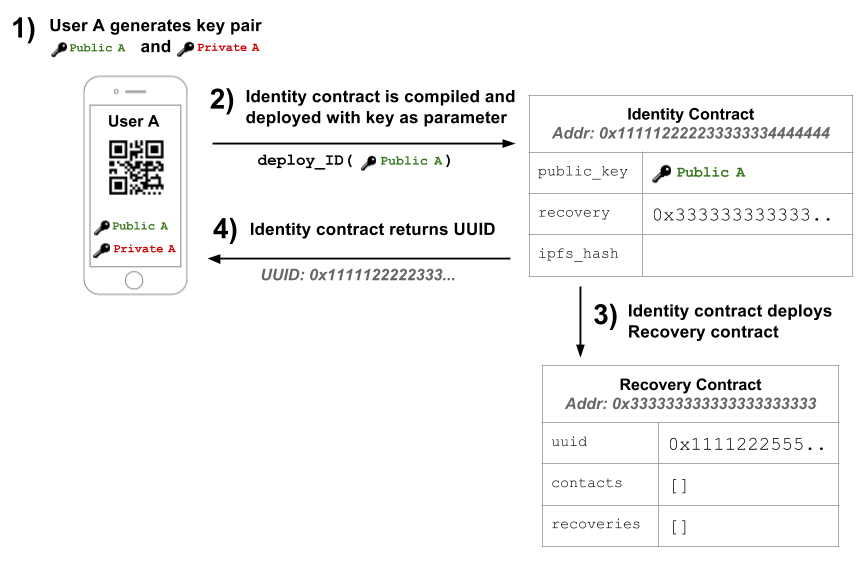
\includegraphics[width=1.0\textwidth]{./images/DiagramSignup.png}
      \caption{Identity Creation: Key generation and contract deploy steps.}
       \label{fig:diagram-signup}
\end{figure}

The steps for identity creation are shown in Figure \ref{fig:diagram-signup}. To create an identity on the platform, the user first generates a public and private key pair on their device. The public key acts as the local identifier for the user and is also an Ethereum address that can hold currency. The private key is used for signing transactions from this address, and to prove ownership of the public key.

The user then compiles a copy of the \textit{Identity Contract} source code and publishes it to the blockchain via their Ethereum address. This transaction returns the Ethereum address to which the contract was deployed, and is used as the unique identifier or \ac{UUID} for the user. 

This form of identifier is seen in the case of uPort in Section \ref{sec:uport}, and it is useful as it functions as both a unique address and a pointer to the contract data on the blockchain.

The identity contract itself also publishes a second contract, known as the \textit{Recovery contract}. This contains the storage and logic for identity recovery using a consensus of the user's selected friends.


\subsection{User Attributes}
These are descriptive attributes relating to the user, for example, their name, address or date of birth. These are stored as \ac{JSON} objects on the decentralised storage platform \ac{IPFS}. To store a user's attributes on their identity, they upload it to \ac{IPFS} and receive a resultant hash pointing to the content on the \ac{IPFS} network. The user can then send a signed transaction using their device public key to their identity contract which updates the \ac{IPFS} hash.

\subsection{Attribute Signing}
Information about a user is not useful unless it is verified by a trusted third party. A user can request that a third party signs their attributes, and can then save the resultant signature with the rest of their identity details. Signatures contain the requested attribute, the \ac{UUID} of the user, and a signature expiry time. 

Smart contracts currently cannot perform signing functions on arbitrary pieces of text, and therefore the signatures must be done using the private key on the third party's device. Signatures performed using device keys are accompanied by the associated contract address for subsequent verification.

There is, therefore, a link between the user's device keys and the \ac{UUID} value stored on the blockchain that must be consistently verified. All signed data must be checked against the blockchain to ensure that the public key used to sign is still matched with the correct identity.

\subsection{Attribute Disclosure}
\label{sec:attribute-disclosure}
\begin{figure}[ht]
\centering
     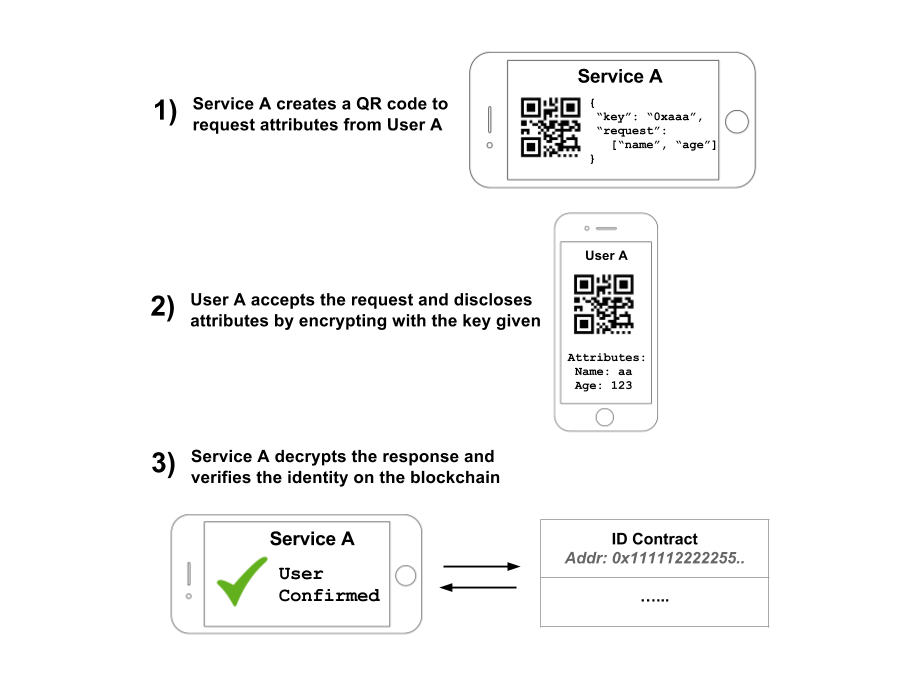
\includegraphics[width=1.0\textwidth]{./images/DiagramDisclosure.png}
      \caption{Attribute Disclosure: Steps to disclose user attributes to a third party.}
       \label{fig:diagram-disclosure}
\end{figure}
To disclose a user's attributes to another party, the third party service creates a disclosure request with the required attributes. This is shown in the first step of Figure \ref{fig:diagram-disclosure}. When the user receives this request on the device, they can confirm or deny the disclosure of the requested data.

The user then encrypts the attributes and any associated signatures with the third party's public key. The user also signs the request with the private key on their device and sends over the result.

The receiving party then decrypts this message and verifies that the public key used to create the signature is linked to the correct identity on the blockchain. The validity of any attribute signatures is also verified by querying the blockchain and checking that the signing parties are trusted.

Attributes of a user can only be considered valid if they are accompanied by attestations from third parties that are trusted by the receiver. An extension to this solution would allow a chain of trust to be created that links entities to trusted roots. Listing the public keys of trusted parties on an online service like the MIT PGP Public Key Server \cite{massachusetts_institute_of_technology_mit_nodate} could facilitate this approach.

\subsection{Identity Recovery}
\label{sec:identity-recovery}
\begin{figure}[ht]
\centering
     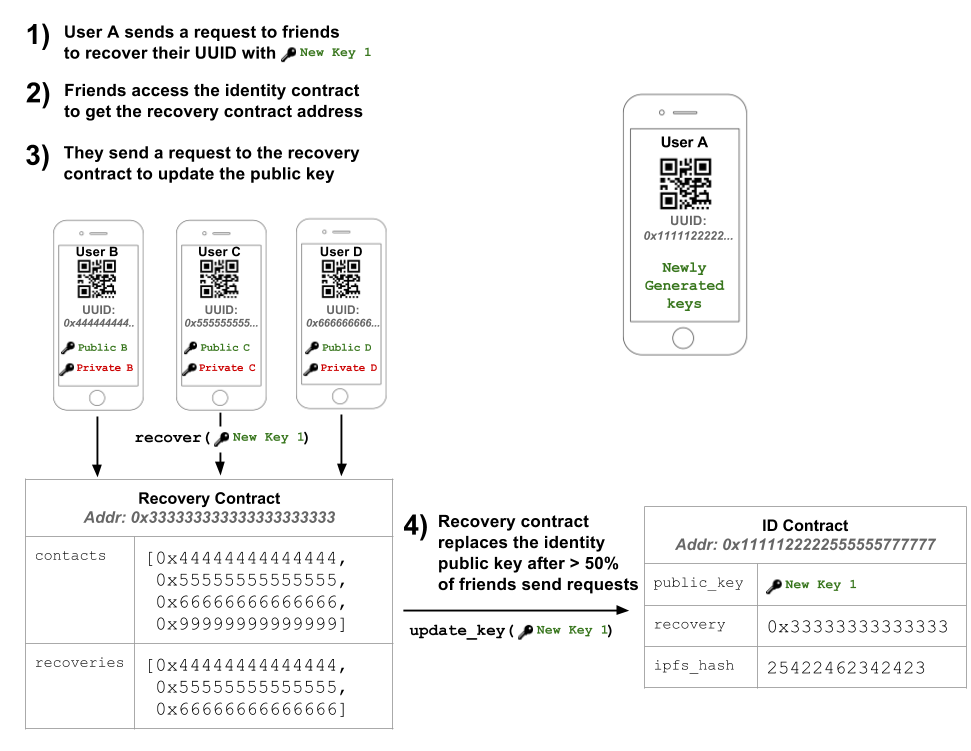
\includegraphics[width=1.0\textwidth]{./images/DiagramRecovery.png}
      \caption{Identity Recovery: Steps to recover an identity using a network of trusted peers.}
       \label{fig:diagram-recovery}
\end{figure}

Recovery is a vital part of enabling public key cryptography for general use \cite{microsoft_key_nodate}.
In this approach, users preselect a group of recovery contacts to facilitate reinstatement of the user's identity in the event of key loss or compromise. The list of contacts are stored in the recovery contract connected to the user's identity. 

If a user needs to recover their identity, they first generate a new set of public and private keys. This can be seen in Step 1 of Figure \ref{fig:diagram-recovery} above. The user then meets with their contacts and asks them to send recovery requests containing their new public key.

The contacts then access the user's associated identity contract to get the address of the recovery contact before sending the request. The recovery contract stores pending requests, and has the power to make the key change once a majority decision is reached.

\subsection{Key Revocation}
Key revocation is used to permanently retire signing and encryption keys from usage \cite{brooks_key_1995}. In the context of key loss or compromise, this is an essential function to prevent malicious actors from abusing the system.

As the user's identity contract and \ac{UUID} is inherently tied directly to their device public key, this is the only valid mapping between these two values. This mapping is verified upon each signature and disclosure request, so separate key revocation does not need to be built into the system.

Key rotation within a user's identity should be logged for archival purposes, so that expired signatures can be verified as being valid at some point in the past. This can be achieved with Ethereum Event Logs \cite{chow_technical_2016}, which act as a logging tool for smart contracts that is cheaper than internal storage. Parties can subscribe to the outputs of these events and be notified when they are announced.

The invalidation of old signatures when an identity has its keys rotated is necessary to maintain the integrity of the identity network. New valid signatures should be distributed to appropriate parties when a relevant key change occurs.
\chapter{Implementation}
\label{chp:implementation}
\section{Components}
\subsection{Web3 Framework}
Web3.js \cite{ethereum_foundation_web3.js_nodate} is a JavaScript interface for Ethereum which conforms to the Generic \ac{JSON} \ac{RPC} Specification \cite{ethereum_foundation_ethereum_nodate} used by other Ethereum clients. It can send transactions, call functions in smart contracts and compile and deploy Solidity smart contract code.

Web3 was chosen as the interface for interacting with the Ethereum smart contracts, as it is a platform-independent framework that operates client-side and within the browser. Web3 can use a local Ethereum node for testing purposes, or it can be pointed at a remote node connected to the Ethereum \textit{Test Net} or \textit{Main Net}. Infura \cite{noauthor_infura_nodate} is a service that offers public Ethereum nodes that serves blockchain \ac{RPC} requests for applications.

\subsection{Transaction Signing}
Transaction signing is not offered by Web3, but it can be offloaded to the connected Ethereum node if the keys of the requested account are stored on the node. To enable local transaction signing in the client, packages like ethereumjs-tx \cite{noauthor_ethereumjs-tx_nodate} and ethereumjs-util \cite{noauthor_ethereumjs-util_nodate} can be added to the project. These packages use private keys stored locally to sign transaction requests, and they subsequently send raw transactions to the Ethereum node.

Metamask \cite{noauthor_metamask_nodate} is another project for Ethereum account management that runs as a browser extension. It stores the public and private keys for Ethereum wallets in the browser local storage and supports client-side transaction signing.

\subsection{TestRPC}
TestRPC \cite{noauthor_testrpc_nodate} can be used for rapid testing of Ethereum smart contracts and applications. It simulates a full Ethereum node and local blockchain network. It can generate a number of addresses with initial balances and store their keys on the node. It also mines blocks of transactions instantly to facilitate faster development.

The implementation of this project uses TestRPC, but it could be easily changed to point to an Ethereum node connected to the live blockchain. TestRPC was convenient as it gave generated wallets initial account balances, which removed the need for mining Ether to fund contract deployments and transactions.

\subsection{IPFS}
A local \ac{IPFS} node was set up to store user identity data during development. This could also be easily pointed to a public \ac{IPFS} node such as one hosted by the organisation themselves.

Data on \ac{IPFS} follows a standard format for storing attributes and signatures. An example is shown below.

\begin{spacing}{1}
  \inputminted{json}{./code/IPFS.json.txt}
\end{spacing}
Example snippet hash: \textit{QmUHxAMb53UeAY6srn9xEBUthcBVT5sVrRRJrbwwkqxy3Z}.

\section{Interface}
\subsection{Main Screen}
The primary interface of the implementation is shown below in Figure \ref{fig:home-screen}. It displays the user's \ac{UUID}, their name attribute, Ethereum wallet balance, device public key, recovery contract address and \ac{IPFS} content hash.

\begin{figure}[ht]
\centering
     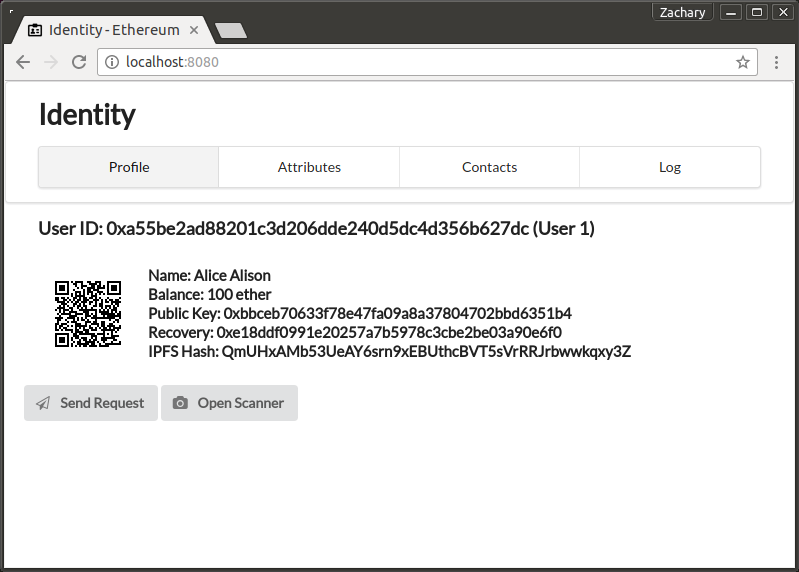
\includegraphics[width=1.0\textwidth]{./images/HomeScreen.png}
      \caption{Home Screen: Initial view of a user's identity on the platform.}
       \label{fig:home-screen}
\end{figure}

The \ac{UUID}, which is also the address of the user's identity contract, is stored in the local storage of the browser. This is then used to fetch the rest of the user's data.

\subsection{Data Transfer}
\label{sec:data-transfer}
QR codes were chosen as the transport protocol to transfer information between parties in the system. This can be replaced with any other peer-to-peer messaging protocol like Bluetooth or Wi-Fi Direct. Ethereum has plans to release a dedicated protocol known as Whisper  \cite{ethereum_foundation_whisper_nodate} which could also be used in the future.

An example of the QR code used to transmit a signature request is shown in Figure \ref{fig:signature-request} below. This shows the accompanying \ac{JSON} value that contains the user's \ac{UUID}, the name of the attribute to be signed, and the value. This can be scanned by a third party, approved, and then the attributes signed and returned.

\begin{figure}[ht]
\centering
     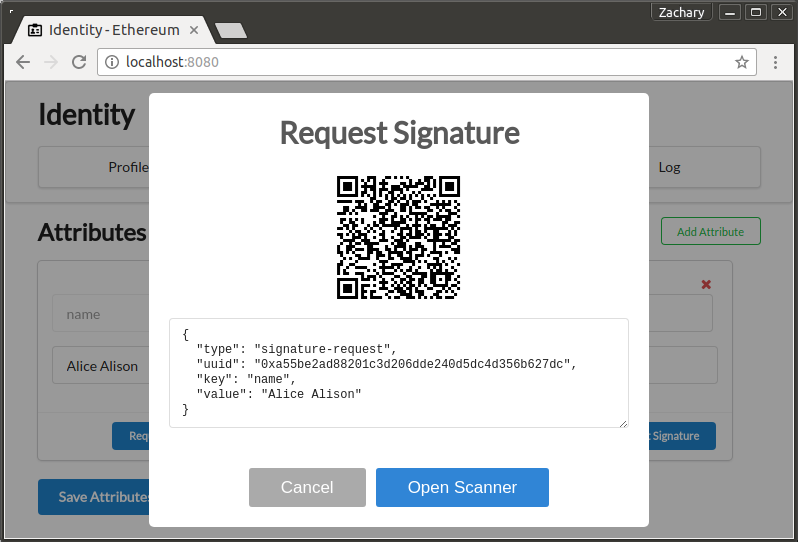
\includegraphics[width=1.0\textwidth]{./images/SignatureRequest.png}
      \caption{Signature Request: An example using a QR code to request a signature.}
       \label{fig:signature-request}
\end{figure}

A table of the possible message types is also shown in Table \ref{tab:message-types} below. These are read by the JavaScript implementation and present different dialog boxes to the user.

\begin{table}[H]
	\centering
    \begin{tabular}{|p{4cm}|p{8cm}|}
       \hline \textbf{Message Type} & \textbf{Attributes} \\
       \hline contact-card & uuid \\
       \hline signature-request & uuid, key, value \\
       \hline attribute-request & attributes, uuid \\
       \hline recovery-request & uuid, new-key \\
       \hline signature-result & key, value, signer, signature \\
       \hline disclosure-result & uuid, attributes, signature \\
       \hline
    \end{tabular}
    \caption{Message types and values for passing data between users.}
    \label{tab:message-types}   
\end{table}

\section{Additional Features}
\subsection{Deterministic Wallet Seed}
Another recovery mechanism that could be added to the system is a recovery mnemonic, a human readable seed that is used to generate the public and private key pair.

A \ac{BIP} known as \ac{BIP}39 \cite{noauthor_bip-0039_nodate} was released in 2013 to help users make a backup of their digital currency wallets. It builds upon the advancements of deterministic wallet generation from a given seed brought about by \ac{BIP}32 \cite{noauthor_bip-0032_nodate}.

A twelve or sixteen-word seed is generated from a list of 2048 English words. This mnemonic is then hashed and converted into a seed value for the key generation function. \textit{Hierarchical Deterministic} wallets allow an infinite amount of addresses to be generated from a given seed, using an index value.

Human readable seeds can thus be given to the user to write down on paper, and they allow multi-currency addresses to be recovered. This should act as the primary backup feature for the user's identity, as it is simpler than coordinating with multiple backup contacts.


\subsection{User Attribute Privacy}
\label{sec:user-attribute-privacy}
User attributes are stored unencrypted on \ac{IPFS} and linked directly to the user's \ac{UUID}. This means that whenever the \ac{UUID} is shared, the receiving party can view all the public attributes and signatures relating to that user. Other existing implementations such as uPort as seen in Section \ref{sec:uport} allow the use of privately stored attributes that are not on the blockchain, but recovery of these is not possible in cases of device compromise.

A proposed solution is to have a second "encryption key" in addition to the device signing key owned by the user. This encryption key would be used to encrypt all user data before publishing it to the public blockchain. Disclosure of attributes is done by downloading this encrypted data, and then decrypting it before encrypting with the receivers public key for transport.

As private data cannot be stored in Ethereum smart contracts, the encryption key is not recoverable using the blockchain. The function of storing encrypted data in smart contracts that they can act on is known as secure multi-party computation \cite{andrychowicz_secure_2014} and remains largely unsolved for blockchain technology. Some facility is therefore required to enable recovery contacts to restore a user's encryption key, to avoid them losing their stored private data.

\textit{Threshold cryptography} \cite{desmedt_threshold_1994} is proposed to solve this, which allows a piece of data to be split such that M of N pieces need to be combined to restore it. It allows secure sharing of a secret value such that no less than the specified number of peers can come together to reveal the data.

The private encryption key of the user could, therefore, be split using the threshold cryptography algorithm, and encrypted with the public keys of the user's recovery contacts. In the event of key loss or compromise, the user can request the decrypted values from M of N contacts and then run the data back through the algorithm to restore their private key.
\chapter{Security Evaluation}
\section{Attack Considerations}
The security aspects of a system are especially relevant in the identity space, as \ac{PII} that is hacked or leaked can have a detrimental effect on both users and companies \cite{acquisti_is_2006}. 

This section documents some possible attack vectors for the implementation in this paper, and the solutions proposed to counteract them. These are considered \textit{active attacks}, where the attacker is attempting to alter the live operation of the system. They are distinct from \textit{passive attacks} where the attacker is attempting to merely obtain data for later use.

\subsection{Disclosure Replay Attack}
When user attributes are disclosed to a third party, they could be susceptible to a \textit{message replay} or \textit{playback attack} if the response is logged and replayed at a later time. This could lead to identity impersonation as the signed response can be verified as valid \cite{noauthor_replay_nodate}.

A solution to this is for the requesting party to present a random string known as a \textit{challenge} to the user. The user must sign this challenge with their private key. Upon receipt, this signature can be verified against the challenge string that was sent. These challenge strings are transient and regenerated for each request. 

\subsection{Man-in-the-Middle Attack}
A \textit{man-in-the-middle attack} occurs when an attacker intercepts and alters messages between two parties who are directly communicating with each other. The likelihood of this attack is related to the communication channel chosen by the parties.

The identity system in this paper can only attempt to mitigate this by ensuring that data is encrypted with the receiving party's public key for data privacy, and signed with the sending party's private key for message integrity. The key exchange step of the communication process is assumed to be safe, as the system cannot protect this.

The initial key exchange between parties should be done in person, with visual confirmation that keys transferred are correct. If this information remains unaltered, then future communication through other channels can be considered safe.

\subsection{Multi-User Compromise}
Identity recovery is supported by giving authority to a group of the user's trusted friends. One downside to this approach is that the list of connected friends is stored on the public blockchain, so they could be susceptible to compromise as a group. An attacker only needs to take over 51\% of the user's contacts, which could be a small number if they do not possess very many.

Time-delayed actions are proposed to solve this issue, notably by uPort, with appropriate notification and logging. The Ethereum protocol can output \textit{Event Logs} \cite{chow_technical_2016}, to which other parties can subscribe to receive updates. When the recovery contract receives requests from a user's recovery contacts, it can delay any account changes by a number of days and notify accordingly. 

This can be done by binding actions to the timestamp announced within the block, and ensuring they are not activated unless a specified delay has passed. Incoming transactions to the contract check for pending actions and perform the functions if the correct time has elapsed. This is referred to as lazy execution \cite{merriam_how_2016}, and is required as there is currently no way for a contract to activate itself after a specific amount of time.

\subsection{Sybil Attack}
A \textit{Sybil attack} \cite{douceur_sybil_2002} occurs where a reputation system is undermined by the creation of many forged identities. This can affect the credibility of the system and is exploited by attackers to gain a disproportionate amount of power in the network.

A proposed solution \cite{williams_byzantine_2015} subverts Sybil attacks by adding certain costs to parts of the system:
\begin{itemize}
  \item Entry Cost - Barrier cost for creating an identity
  \item Existence Cost - Continuous fee for having an active identity
  \item Exit Penalty - Penalty fee or dismissal for acting dishonestly
\end{itemize}

The identity system proposed in this paper does not attempt to inherently prevent Sybil attacks, but is architected in the hope that attestations by reputable authorities can bootstrap trust into the network.

The addition of \textit{reputation scores} \cite{josang_survey_2007} given to identities is also a promising solution, which can be used to derive trust from a network of attestations. This is similar to the Web of Trust concept shown in Section \ref{sec:web-of-trust}.
\chapter{Conclusion}
Identity in the digital sphere has been shown in this paper to be important both personally to users, and economically to businesses. The risks and negative effects that centralised identity systems possess imply that they are not a perfect solution for the identity domain.

Decentralised identity systems that take a more user-centric approach pose less risk to the service provider and provide a greater benefit to the end user. This aspect was focused on in the context of blockchain technology, to try and explore a viable and realistic solution to apply to the field.

\section{Research Objectives}
A number of research objectives were outlined at the start of this paper, with the view of evaluating their feasibility and relevance in the proposed solution. They are assessed under the headings below.

\subsubsection{Data Security}
The aim of this requirement is to ensure that user information kept secure and private. The approach proposed in this paper ensures data security in transit using encryption in Section \ref{sec:data-transfer}. It also presents a novel approach to ensuring data at rest is kept private, using threshold cryptography with an encryption key as detailed in Section \ref{sec:user-attribute-privacy}.

\subsubsection{Interface Usability}
The primary focus of the interface design was to abstract away the fine details of public and private key creation, management and usage from the user. This was achieved in part by ensuring that key generation is done automatically with identity creation, and key storage was managed by the client application. Key recovery is also facilitated by the recovery quorum process detailed in Section \ref{sec:identity-recovery}, which removes the requirement of careful key management by the user.

\subsubsection{Identity Verifiability}
The attribute signing and signature verification processes detailed in Section \ref{sec:attribute-disclosure} guarantee that identities can be securely validated. A careful note can be made about the validity of user attributes, as these are only as trusted as the entities that provide the associated attestations. Even though attestations might be cryptographically valid, the network cannot verify \textit{why} the claim has been made. Lists of trusted authorities should be cautiously monitored to maintain a high level of trust in the network.

\subsubsection{Account Recovery}
The proposed system supports identity recovery using a network of peers, which is robust to single user compromise. An approach is also shown to recover private identity data if the keys are distributed correctly between these trusted peers.

\subsubsection{Self-Sovereignty}
The self-sovereign approach to identity management is fundamental to this research, and providing full autonomy over a user's identity and associated data helps to accomplish this. By giving the user sole identity access and the power to delegate authority to peers, users are no longer dependent on third parties for managing or storing their data. The blockchain element is crucial for this complete data decentralisation, as it is one of the few technologies that fundamentally supports it.

\section{Future Work}
Although this paper presents a comprehensive design and proof-of-concept implementation of a self-sovereign identity system; there are still improvements that can be made as the technology matures. 

\subsection{Metropolis Release}
The Ethereum blockchain is due to release a protocol upgrade soon, which will bring about improvements in transactions and smart contract operation.

Work on allowing smart contracts to pay the transaction fees for users could be included, which would remove the requirement for users to have an initial Ethereum balance before joining the system. This is currently tackled by uPort by using a \textit{currency faucet} to pay these fees \cite{noauthor_does_nodate}, but by doing so, it introduces an element of external dependency in the system.

RSA signature verification could also be added to this release, and it has been discussed in a recent proposal \cite{noauthor_eip0074_nodate}. This would remove the dependency on the client for identity verification and allow it to be done transparently on the blockchain.

\bibliographystyle{IEEEtran}
\bibliography{Zotero}

\begin{appendix}
  \addcontentsline {toc}{chapter}{Appendices}
  \chapter{Contract Source Code}

\begin{spacing}{1}
  \section{Identity Contract}
  \label{apd:identity-contract}
  \inputminted{C}{./code/Identity.sol.txt}

  \section{Recovery Contract}
  \label{apd:recovery-contract}
  \inputminted{C}{./code/Recovery.sol.txt}
\end{spacing}

\section{Project Repository}
The source code for the proof-of-concept system outlined in this paper can be found on GitHub at \url{https://github.com/zachd/ethereum-identity-research}. 

The final commit hash is \texttt{82eeef2c64a2e3dbc0c286c81a8f215d7ee2a8d0}.
\end{appendix}

\end{document}